\section{Introduction}

Ce projet se penche sur la possibilité de classifier les aéroports par pays à partir d'un graphe non orienté où les sommets sont les aéroports et les arêtes les routes aériennes. Pour cela nous utiliserons tout au long des expérimentations un modèle GCN (Graph Convolutional Network) qui est un modèle de deep learning spécialisé pour les graphes.\\
Nous nous intéressons particulièrement à l'influence de différents facteurs sur la performance de la classification, tels que la position géographique des aéroports, la population des villes desservies et la structure du graphe de connexions aériennes. Notre hypothèse principale est que l'ajout d'informations démographiques, en complément des données géographiques, améliorera la précision de la classification.  Pour valider cette hypothèse, nous allons réaliser une série d'expérimentations en utilisant différentes configurations d'attributs et de structures de graphe,  et en évaluant les performances de différents algorithmes de classification.\\

Pour visualiser les résultats, nous utiliserons un affichage spaciale que nous comparerons à la carte suivante représentant les aéroports classifiés par pays.\\

\begin{figure}[h!]
    \centering
    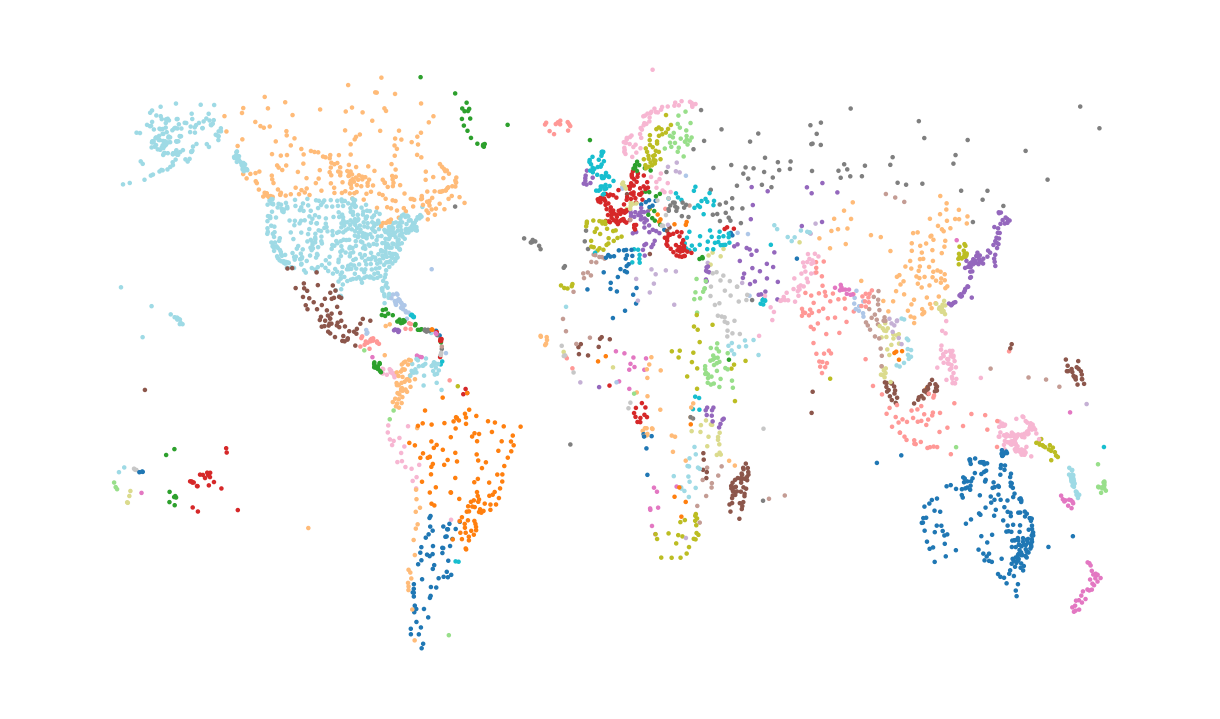
\includegraphics[width=\textwidth]{content/img/map-airports-goal.png}
    \caption{Carte des aéroports classifiés par pays (objectif)}
    \label{fig:map}
\end{figure}
